%% BioMed_Central_Tex_Template_v1.06

%%% additional documentclass options:
%  [doublespacing]
%  [linenumbers]   - put the line numbers on margins

%%% loading packages, author definitions

%\documentclass[twocolumn]{bmcart}% uncomment this for twocolumn layout and comment line below
\documentclass{configs/bmcart}

%%% Load packages
%\usepackage{amsthm,amsmath}
%\RequirePackage{natbib}
%\RequirePackage[authoryear]{natbib}% uncomment this for author-year bibliography
%\RequirePackage{hyperref}
%\usepackage[utf8]{inputenc} %unicode support
%\usepackage[applemac]{inputenc} %applemac support if unicode package fails
%\usepackage[latin1]{inputenc} %UNIX support if unicode package fails
\usepackage{booktabs}
\usepackage{graphicx}
\usepackage{hyperref}
\hypersetup{
    colorlinks=false,
    linkcolor=black,
    filecolor=black,      
    urlcolor=black,
}
\usepackage{url}
\usepackage{amsmath} % small matrix package
\usepackage[acronym]{glossaries}

%\makenoidxglossaries
\makeglossaries
\newacronym{roi}{ROI}{region of interest}
\newacronym{sfm}{SfM-MVS}{structure-from-motion multi-view stereo photogrammetry}
\newacronym{dom}{DOM}{digital orthophoto map}
\newacronym{dsm}{DSM}{digital surface model}
\newacronym{lidar}{LiDAR}{light detection and ranging}
\newacronym{ml}{ML}{machine learning}
\newacronym{dl}{DL}{deep learning}
\newacronym{pcd}{PCD}{point cloud data}
\newacronym{gis}{GIS}{geographic information system}
\newacronym{gcp}{GCPs}{ground control points}
\newacronym{mtp}{MTPs}{manual tie points}
\newacronym{mkl}{MKL}{math kernel library}
\newacronym{gui}{GUI}{graphical user interface}
\newacronym{iou}{IoU}{intersection of union}
\newacronym{rtk}{RTK}{real-time kinematic}
\newacronym{pmvs}{PMVS}{patch-based multi-view stereo}
\newacronym{pcl}{PCL}{point cloud library}


%%%%%%%%%%%%%%%%%%%%%%%%%%%%%%%%%%%%%%%%%%%%%%%%%
%%                                             %%
%%  If you wish to display your graphics for   %%
%%  your own use using includegraphic or       %%
%%  includegraphics, then comment out the      %%
%%  following two lines of code.               %%
%%  NB: These line *must* be included when     %%
%%  submitting to BMC.                         %%
%%  All figure files must be submitted as      %%
%%  separate graphics through the BMC          %%
%%  submission process, not included in the    %%
%%  submitted article.                         %%
%%                                             %%
%%%%%%%%%%%%%%%%%%%%%%%%%%%%%%%%%%%%%%%%%%%%%%%%%

%\def\includegraphic{}
%\def\includegraphics{}


%%% Put your definitions there:
%\startlocaldefs
%\endlocaldefs


%%% Begin ...
\begin{document}

%%% Start of article front matter
\begin{frontmatter}

\begin{fmbox}
\dochead{Software}

%%%%%%%%%%%%%%%%%%%%%%%%%%%%%%%%%%%%%%%%%%%%%%
%%                                          %%
%% Enter the title of your article here     %%
%%                                          %%
%%%%%%%%%%%%%%%%%%%%%%%%%%%%%%%%%%%%%%%%%%%%%%

\title{EasyRIC: A python package for annotation transformation among 3D reconstruction products}

%%%%%%%%%%%%%%%%%%%%%%%%%%%%%%%%%%%%%%%%%%%%%%
%%                                          %%
%% Enter the authors here                   %%
%%                                          %%
%% Specify information, if available,       %%
%% in the form:                             %%
%%   <key>={<id1>,<id2>}                    %%
%%   <key>=                                 %%
%% Comment or delete the keys which are     %%
%% not used. Repeat \author command as much %%
%% as required.                             %%
%%                                          %%
%%%%%%%%%%%%%%%%%%%%%%%%%%%%%%%%%%%%%%%%%%%%%%

\author[
   addressref={aff1},
   %email={haozhou-wang@g.ecc.u-tokyo.ac.jp}
]{\inits{HW}\fnm{Haozhou} \snm{Wang}}
\author[
   addressref={aff1},
   corref={aff1}, 
   email={guowei@g.ecc.u-tokyo.ac.jp}
]{\inits{WG}\fnm{Wei} \snm{Guo}}

%%%%%%%%%%%%%%%%%%%%%%%%%%%%%%%%%%%%%%%%%%%%%%
%%                                          %%
%% Enter the authors' addresses here        %%
%%                                          %%
%% Repeat \address commands as much as      %%
%% required.                                %%
%%                                          %%
%%%%%%%%%%%%%%%%%%%%%%%%%%%%%%%%%%%%%%%%%%%%%%

\address[id=aff1]{
  \orgname{ International Field Phenomics Research Laboratory, Institute for Sustainable Agro-ecosystem Services, Graduate School of Agricultural and Life Science, The Univerisity of Tokyo}, 
  \postcode{188-0002} 
  \city{Tokyo}, 
  \cny{Japan}
}

%%%%%%%%%%%%%%%%%%%%%%%%%%%%%%%%%%%%%%%%%%%%%%
%%                                          %%
%% Enter short notes here                   %%
%%                                          %%
%% Short notes will be after addresses      %%
%% on first page.                           %%
%%                                          %%
%%%%%%%%%%%%%%%%%%%%%%%%%%%%%%%%%%%%%%%%%%%%%%

%\begin{artnotes}
%%\note{Sample of title note}     % note to the article
%\note[id=n1]{Equal contributor} % note, connected to %author
%\end{artnotes}

\end{fmbox}% comment this for two column layout

%%%%%%%%%%%%%%%%%%%%%%%%%%%%%%%%%%%%%%%%%%%%%%
%%                                          %%
%% The Abstract begins here                 %%
%%                                          %%
%% Please refer to the Instructions for     %%
%% authors on http://www.biomedcentral.com  %%
%% and include the section headings         %%
%% accordingly for your article type.       %%
%%                                          %%
%%%%%%%%%%%%%%%%%%%%%%%%%%%%%%%%%%%%%%%%%%%%%%

\begin{abstractbox}

\begin{abstract}
\parttitle{Background} 
Applying high-throughput phenotyping technologies in agriculture provides an advanced and efficient method for managing and breeding crops in practical applications. Compared with device-specified remote sensing technologies (laser scanning, \acrfull*{lidar}, etc.), \acrfull*{sfm}, applicable to price friendly RGB digital cameras, has been widely spread use around the world, and many commercial and open-source software are available to implement this task. However, producing good quality of its products, such as \acrfull*{dom}, \acrfull*{dsm}, and point clouds, is quite computation intensive and hard to meet the same precision of original photos. Hence, linking low computation time produced low quality \acrshort*{sfm} products back to original digital images has significant potential to improve the efficiency and precision for data processing, but to the best of our knowledge, no easy-to-use open source tool is available for this object.

\parttitle{Results}
In this study, a pure python package called EasyRIC (easy reconstruction image converter) was developed to link original photos to \acrshort*{sfm} products. The Lotus (\textit{Nelumbo nucifera}) breeding field were used as a show case to demonstrate the following functions: 1) Clipping the \acrfull*{roi} from point clouds and compare them through time series. 2) Clipping the \acrshort*{roi} from \acrshort*{sfm} products to raw images. 3) Generate bunch of training data in raw images from a few manual marked \acrshort*{roi}.

\parttitle{Conclusions}
This python package shows the great potential to integrate the high-quality original images with  \acrshort*{sfm} produced products. The quick produced low quality products are also acceptable which saved plenty computation time. Also this tool can be used to generate bunch of training data for machine learning with a few manual operation.

\end{abstract}

%%%%%%%%%%%%%%%%%%%%%%%%%%%%%%%%%%%%%%%%%%%%%%
%%                                          %%
%% The keywords begin here                  %%
%%                                          %%
%% Put each keyword in separate \kwd{}.     %%
%%                                          %%
%%%%%%%%%%%%%%%%%%%%%%%%%%%%%%%%%%%%%%%%%%%%%%

\begin{keyword}
\kwd{3D reconstruction}
\kwd{Orthomosaic}
\kwd{Training data generation}
\kwd{Phenotyping}
\kwd{Open source}
\kwd{Pix4D}
\end{keyword}

\end{abstractbox}
%
%\end{fmbox}% uncomment this for twocolumn layout

\end{frontmatter}

%%%%%%%%%%%%%%%%%%%%%%%%%%%%%%%%%%%%%%%%%%%%%%
%%                                          %%
%% The Main Body begins here                %%
%%                                          %%
%% Please refer to the instructions for     %%
%% authors on:                              %%
%% http://www.biomedcentral.com/info/authors%%
%% and include the section headings         %%
%% accordingly for your article type.       %%
%%                                          %%
%% See the Results and Discussion section   %%
%% for details on how to create sub-sections%%
%%                                          %%
%% use \cite{...} to cite references        %%
%%  \cite{koon} and                         %%
%%  \cite{oreg,khar,zvai,xjon,schn,pond}    %%
%%  \nocite{smith,marg,hunn,advi,koha,mouse}%%
%%                                          %%
%%%%%%%%%%%%%%%%%%%%%%%%%%%%%%%%%%%%%%%%%%%%%%

\section*{Background}
Para1: Agricultural crisis -> demand for high-throughput phenotyping

Para2: Common high-throughput phenotyping technologies -> why RGB SfM

Para3: SfM background, \textbf{algorithm}, and software (computation intensive drawbacks, need low quality to save time)

Para4: Data processing (the difficulties to of use the result of SfM, e.g. 1) low quality of DOM make canopy cover, organ detection. -> link to raw image; 2) 3D analysis not easy (require large RAM and good computation to processing point cloud, and the quality of point cloud couldn't too large -> 3D to 2d, 3D clipping, there is no common tool to make this transfer easy)

Para5: 4D time series analysis demand and point cloud clipping

Para6: Training Data crisis

Para7: Objectives

\section*{Implementation}

This study implemented a open-source python package called EasyRIC (easy reconstruction image converter) to cropping \acrshort*{sfm} software (e.g. Pix4Dmapper, Agisoft Metashape, etc.) produced products based on \acrfull*{roi} and linking them on original images. Though the source codes were cross-platform due to the characteristic of python language, they were programmed and tested under Windows 10 64-bit platform and Intel CPU with \acrfull*{mkl} support. For the package performance reliability, the 8GB of RAM and CPU with at 3.0 GHz are recommended. The requirements to use this packages requires: the Python >= 3.7, numpy >= 1.18.1, scikit-image >= 0.16.2, opencv-python >= 3.4.2.16, pyproj == 2.6.1.post1, pyparsing >= 2.0.1 are required, and following pure python packages were included in source code without installation: pyshp, Send2Trash, ezdxf, and plyfile. The user manual and source code can be accessed via: \url{https://github.com/HowcanoeWang/EasyRIC} and the License is GPL-3.0 which is free to use for any purpose, forever.

The general workflow of this tool was shown in Figure \ref{fig:workflow}. There were three main parts of this workflow, including two input data preparations: 3D reconstruction outputs (Figure \ref{fig:workflow}.a) and corresponding \acrfull*{roi} by other tools (Figure \ref{fig:workflow}.b); and EasyRIC converting tool core functions (Figure \ref{fig:workflow}.c). Each part had tight correspondence with 3D reconstruction workflow, and was split into (1) SfM stage, (2) MVS stage, and (3) GIS stage respectively. 

The first SfM stage (Figure \ref{fig:workflow}.c-1) provides the experimental function that convert the \acrfull*{roi} on one raw images (2D) to the other raw images (2D) just after SfM stages ("2D to 2D") in \acrlong*{sfm} software without further time-consuming MVS densification and GIS outputs steps. It saves a plenty of time in data processing, however, our case study pre-experiment result (Additional file 1) showed this experimental stage still needs some improvements to make the accuracy acceptable without double ROI making.

The second MVS stage (Figure \ref{fig:workflow}.c-2) transforms the \acrfull*{roi} on point cloud data (3D) to the related raw images (2D) after MVS densification in \acrlong*{sfm} software ("3D to 2D"). It also enables the clipping function of point cloud data within given \acrshort*{roi}, which could help increase the feasibility of data analysis and decrease the storage space.

The third GIS stage (Figure \ref{fig:workflow}.c-3) transforms the \acrfull*{roi} on \acrfull*{gis} products to related raw images (2D). Commonly, the ROI is marked manually by GIS software on \acrfull*{dom}. The height information is provided by \acrfull*{dsm}. Compared with 3D information extracted directly on point clouds, this geometry information is combined by XY axis from DOM and Z axis from DSM, named 2.5D to distinguish with point cloud 3D. This stage is also specified as "2.5D to 2D". Besides, it provides functions of clipping \acrshort*{dom} and \acrshort*{dsm} along \acrshort*{roi} or into given size grids with labels, not only helps the management of data, but also helps the connection to deep learning framework directly.

\subsection*{Input data preparation}

\subsubsection*{Image collection and 3D reconstruction}
% image collection
The good quality of input image data are the fundamental of \acrfull*{sfm} process as well as the EasyRIC package. The images with balanced brightness, exposure, and minimum motion blur are of great importance. Over 50\% overlapping among each adjacent images is also recommended. Though \acrfull*{gcp} or \acrfull*{mtp}, or even \acrfull*{rtk} are optional for \acrshort*{sfm} software. It is strongly recommended to set several object or tags or scalebars to calibrate and define geographic positions. One option is Chilitags (\url{https://github.com/chili-epfl/chilitags}), the automatic workflow decrease a plenty of workload in current \acrshort*{sfm} software.

% SfM workflow
After getting good quality of data, the \acrshort*{sfm} workflow is required.Currently, there are many \acrshort*{sfm} software available, can be split into commercial and open-source two classes. The most often used commercial software include Pix4Dmapper and Agisoft Metashape. For open-source software, including OpenMVG (\url{http://openmvg.readthedocs.io/en/latest}), libMV (\url{https://developer.blender.org/tag/libmv}), VisualSFM (\url{http://ccwu.me/vsfm}), Bundler (\url{http://www.cs.cornell.edu/~snavely/bundler}), FieldReconst (\url{http://cse.naro.affrc.go.jp/rsugiura/FieldReconst}), and so on. Compared with commercial software, most of the open-source software can not deal with the full process of \acrshort*{sfm}, as Zhu et al., \cite{zhu_quantification_2020} and Hui et al,. \cite{hui_image-based_2018} applied in their projects, many software including VisualSFM, \acrfull*{pmvs} \cite{furukawa_accurate_2010}, \acrfull*{pcl} \cite{rusu_3d_2011}, and Geomagic Studio software (Raindrop Geomagic, Morrisville, NC, USA) are used to implement the full process that imbedded in Pix4Dmapper. For this study, the commercial Pix4Dmapper was used as its default setting to produce required camera parameters (pmatrix, external and internal parameters), \acrfull*{pcd}, and GIS products \acrfull*{dom} and \acrfull*{dsm}, and all outputs of Pix4DMapper have been supported and tested. For future, other commercial software or open source software will be supported.

\subsubsection*{Region of Interest (ROI) making}
Currently, the EasyRIC package hasn't provide any \acrfull*{gui} for manual \acrfull*{roi} marking. So different external software to marking ROI on different stage outputs are required.

For the first SfM stage, which requires obtaining 2D pixel coordinates on raw images, common photo processing software can be used, e.g. open-source GIMP or commercial Photoshop, these software displays the pixel coordinate where mouse hover. Then these 2D coordinate can be copied or write to txt file or csv file for EasyRIC importing. Also, other deep learning annotation software which produce json annotation files also supported and recommended, for example, LabelMe (\url{https://github.com/wkentaro/labelme}) has been tested and supported in this package.

For the second MVS stage, which produces 3D \acrfull*{pcd}, the 3D coordinate is required. Common point cloud processing software which can pick point cloud points and get the 3D coordinate of each point could be used (e.g. CloudCompare, MeshLab, etc.). The open-source CloudCompare (\url{http://cloudcompare.org/}) has been tested in this project and support export picked points coordinates to txt file for later usage. The tutorial for using CloudCompare to make ROI can be referred on our package user manual. For future, importing the AutoCAD dxf 3D polygon file will be supported.

For the third GIS stage, which requires obtaining 2D geographic coordinates on DOM and DSM, common \acrfull*{gis} processing software including QGIS (open source) or ArcMap (commercial) can be used to produce required polygon shapefiles (*.shp). The produced shp file can be used as the input for EasyRIC package.

\subsection*{Package Algorithms}
The EasyRIC is a python package without any \acrfull*{gui}, please refer to the document \url{https://www.to.be.continued.org} for detailed package usage. Instead of introducing how the package is used, this section demonstrate how the calculation algorithm implemented.

\subsubsection*{Input and output files}
% supported file types
The input file type required for this package includes: pix4d camera parameters, pix4d joint rotation-translation matrix (pmatrix) file (*.txt), digital images (*jpeg, *png), point cloud data (*.pcd, *.ply, *.xyz), geotiff files (*.tiff, DOM and DSM), polygon shapefile (*.shp), shapefile geographic projection file (*.prj), and in the future, 3D polygon file (*.dxf).

% packages used
Several external python site-packages were used to deal with these files, all these data were stored as \textit{numpy.ndarray} based data structure for faster matrix algebra calculation. The *.txt pure text files can be read into \textit{ndarray} by \textit{numpy} package, as stored an index python class linked to each raw image name. For *.jpeg and *.png files, the \textit{scikit-image.io.imread} module was used to load image into \textit{numpy.ndarray} format. For point cloud files, the \textit{open3d.io.read\_pcd} module was used, and for Pix4Dmapper produced *.ply files, sometimes the color information can not be correctly loaded, the \textit{plyfile} package was used to compensate the color loss. For geotiff file, the \textit{tifffile} package was used to load both image layer data to \textit{numpy.ndarray} and geo-header data which contain the offset, resolution, and geographic projection information, helpful for the transformation between pixel coordinate and geographic coordinate on geotiff images. The *.prj file can be read directly by python but \textit{pyproj} package is used to convert pure text to python geo-projection class, and functioned as a projection convertor once the shp projection was not the same with geotiff projection. For 3D polygon *.dxf file, the \textit{ezdxf} package was used to convert to \textit{numpy.ndarray} polygon.

% clip & output files
By importing all these materials into the EasyRIC package, a clip function is provided to clip both point cloud data and geotiff GIS map into small sectors by given ROI polygon coordinates. Then these sectors could be saved as the same file type into disk, for future use.

\subsubsection*{Camera distortion}
The lens of camera often cause distortion of image collected, and the extreme example for this distortion application is fisheye camera. Therefore, the pixel coordinate position on image can't exactly reflect the real geometry relationship in the real world. Hence, before doing structure from motion, the camera calibration is always required. The commercial software often have build-in camera calibration model, and Pix4D even support save calibrated undistorted images \cite{pix4d_support_menu_2020}. The transform from original distorted images pixel coordinate $(x_d, y_d)$ to corrected undistorted pixel coordinate $(x_u, y_u)$ by Pix4D output camera distortion coefficients (\textit{calibrated\_camera\_parameters.txt} file, radial distortion $(r_1, r_2, r_3)$ and tangential distortion $(t_1, t_2)$) \cite{pix4d_support_how_2020}:

\begin{align}
  \label{eq:px_correct}
  \text{let:} &
  \left\{\begin{array}{lll}
    x_h & = & (x_d - c_x) / f \\
    y_h & = & (y_d - c_y) / f \\
    \sigma & = & x_h^2 + y_h^2 \\
    k      & = & 1 + r_1 \cdot \sigma + r_2 \cdot \sigma^2 + r_3 \cdot \sigma^3 \\
    x_{hd} & = & k \cdot x_h + t_1 \cdot x_h \cdot y_h + t_2 \cdot (\sigma + 2 \cdot x_h^2) \\
    y_{hd} & = & k \cdot y_h + t_2 \cdot x_h \cdot y_h + t_1 \cdot (\sigma + 2 \cdot y_h^2)
  \end{array} \right. \nonumber \\
  \text{then:} &
  \left\{\begin{array}{lll}
    x_u & = & f \cdot x_{hd} + c_x \\
    y_u & = & f \cdot y_{hd} + c_y
  \end{array} \right.
\end{align}

where, $c_x$ and $c_y$ is the image center in pixel, width (horizontal) and length (vertical), respectively. $f$is camera focal length in mm. 

\subsubsection*{Transform ROI from raw to raw: 2D to 2D}
The geometry of transforming \acrfull*{roi} on one image to another image is shown in Figure \ref{fig:workflow}.c-1. Then, transforming a polygon can be simplified to repeat transforming each polygon corner point to another photo. In this geometry, there are two coordinates, one is the real world geographic coordinate ($xyz_{geo}$, unit is m), the other is the raw image pixel coordinate ($xy_{pix}$, unit is pixel). Assuming there are two images, the first image ($raw_1$) is where we use annotation software (e.g. LabelMe) marked ROI, the other image ($raw_2$) is the target image we want this ROI transformed to. The $K_1$ in $xy_{pix}$ coordinate is one \acrshort*{roi} polygon corner point on $raw_1$, this point related to the point ($K'$) in real world, and is record as $K_2$ on $raw_2$. The $r_i (\omega_i, \varphi_i, \kappa_i)$ represents the camera rotation angles \cite{pix4d_support_yaw_2020}, $p_i$ represents the camera position in real world system ($xyz_{geo}$), $w$ and $l$ represents the camera sensor width (horizontal) and length (vertical) in mm, respectively. All previous photo related parameters could be obtained in \textit{calibrated\_camera\_parameters.txt} file.

As the Pix4D document demonstrated \cite{pix4d_support_how_2020}, the transformation from real world point $K' (X, Y, Z)$ to image pixel coordinate $K_i (x_{k_i}, y_{k_i})$ by Equation \ref{eq:px_correct} is:

\begin{align}
  \label{eq:xyz_prime}
  &\begin{cases}
    x_{k_1} = - f \cdot \dfrac{X'}{Z'} + c_x \\
    y_{k_1} = - f \cdot \dfrac{Y'}{Z'} + c_y
  \end{cases} \nonumber \\
  &\text{where, } \nonumber \\
  &\left[
    \begin{array}{c} X' \\ Y' \\ Z' \end{array} 
  \right]
  =
  \mathbf{R_i}^T \cdot
  \left(
    \left[\begin{matrix} X \\ Y \\ Z \end{matrix}\right] - \mathbf{p_i}
  \right)
\end{align}

where, $\mathbf{R_i}$ is the rotation matrix of camera parameters can be loaded from  or calculated by $r_i (\omega_i, \varphi_i, \kappa_i)$ \cite{pix4d_support_how_2020}:

\begin{align}
  \mathbf{R_i} & = \mathbf{R}_{x_i}(\omega_i) \mathbf{R}_{y_i}(\varphi_i) \mathbf{R}_{z_i}(\kappa_i) \nonumber\\
  & =
    \left[ 
      % amsmath package is required
      \begin{matrix} 
        1 & 0             & 0 \\
        0 & cos(\omega_i) & -sin(\omega_i) \\
        0 & sin(\omega_i) & cos(\omega_i)
      \end{matrix} 
    \right] 
    \left[ 
      \begin{matrix} 
        cos(\varphi_i)  & 0 & sin(\varphi_i) \\
        0               & 1 & 0 \\
        -sin(\varphi_i) & 0 & cos(\varphi_i)
      \end{matrix} 
    \right] 
    \left[ 
      \begin{matrix} 
        cos(\kappa_i) & -sin(\kappa_i) & 0 \\
        sin(\kappa_i) & cos(\kappa_i)  & 0 \\
        0             & 0              & 1
      \end{matrix} 
    \right] \nonumber %\\
  %& = 
  %  \left[ 
  %    \begin{matrix} 
  %      cos(\kappa_i)cos(\varphi_i) 
  %        & -sin(\kappa_i)cos(\varphi_i) 
  %        & sin(\varphi_i) \\
  %
  %      cos(\kappa_i)sin(\omega_i)sin(\varphi_i) + sin(\kappa_i)cos(\omega_i)
  %        & cos(\kappa_i)cos(\omega_i) - sin(\kappa_i)sin(\omega_i)sin(\varphi_i)
  %        & -sin(\omega_i)cos(\varphi_i) \\
  %
  %      sin(\kappa_i)sin(\omega_i) - cos(\kappa_i)cos(\omega_i)sin(\varphi)
  %        & sin(\kappa_i)cos(\omega_i)sin(\varphi_i) + cos(\kappa_i)sin(\omega_i) 
  %        & cos(\omega_I)cos(\varphi_i)
  %    \end{matrix} 
  %  \right] 
\end{align}

However, previous $K' (X, Y, Z)$ to pixel $k_i (x_{k_i}, y_{k_i})$ calculation is a dimension reduction step with Z information loss, which is not reversible. Transforming from given pixel coordinate $k_1$ back to real world $K'$ (revert Equation \ref{eq:xyz_prime} and \ref{eq:px_correct}) could only get the equation with $Z_1'$ as parametric:

$$
  K' = 
  \begin{bmatrix}
    \begin{matrix}
      X \\ Y \\ Z
    \end{matrix}
  \end{bmatrix} 
  = 
  \mathbf{R}^{T^{-1}} \cdot 
  \begin{bmatrix}
    \begin{matrix}
      X' \\ Y' \\ Z'
    \end{matrix}
  \end{bmatrix} + T_1
  =
  \mathbf{R}^{T^{-1}} \cdot Z_1'
  \begin{bmatrix}
    \begin{matrix}
      \dfrac{x_{1center} - x_{k1}}{f} \\ \dfrac{y_{1center} - y_{k1}}{f} \\ 1
    \end{matrix}
  \end{bmatrix} + T_1
$$

It means without knowing the exact value of $Z_1'$, previous step will produce a line rather than a specific point in the real world as well as on the other image, in this case, the most accurate method is marking the ROI on two images, and then calculate their route intersection to get the exact $Z'$ value of $K'$ in real world, then the follow Equation \ref{eq:xyz_prime} to get the pixel coordinate on the third image. 

\subsubsection*{Transform ROI from PCD to raw: 3D to 2D}
When it comes to point clouds (Figure \ref{fig:workflow}.c-2), the Pix4D software will automatically produce \acrfull*{pcd} with XYZ value in geographic coordinates ($PCD_{xyz}$), in this case, the original XYZ often quite large, for UTM zone 54N projection is around (360000, 4000000). To significantly decrease the file size of PCD, it produces an \textit{offset.xyz} file which minus all points with this offset $(X_{offset}, Y_{offset}, Z_{offset})$. Hence the ROI coordinate $(X_{roi}, Y_{roi}, Z_{roi})$ marked in Pix4D produced point cloud need to add this offset to be the real world coordinate $(X_{real}, Y_{real}, Z_{real})$, but it is software dependent, Agisoft support export PCD with original data without offset.

After getting 3D coordinate in real world, the 3D ($xyz_{geo}$) to 2D ($xy_{pix}$) calculation can be conducted by Equation \ref{eq:xyz_prime}, or if perspective lens cameras are used (not fisheye or spherical camera), the joint rotation-translation matrix (pmatrix) which calculated by Pix4D could be directly used to do this calculation \cite{pix4d_support_what_2020}:

$$
\begin{bmatrix}\begin{matrix} x \\ y \\ z\end{matrix}\end{bmatrix}
= PMat_{3\times4} \cdot 
\left(\begin{bmatrix}\begin{matrix} 
  X_{real} \\ Y_{real} \\ Z_{real} \\ 1
\end{matrix}\end{bmatrix} 
- 
\begin{bmatrix}\begin{matrix} 
  X_{offset} \\ Y_{offset} \\ Z_{offset} \\ 1
\end{matrix}\end{bmatrix}
\right)
$$

\subsubsection*{Transform ROI from GIS map to raw: 2.5D to 2D}
As shown in Figure \ref{fig:workflow}.c-3), the \acrfull*{roi} of GIS coordinates often stored as shapefile polygon (*.shp), it could be loaded by previous $input and output files$ section. However, sometimes the projection of shapefile are not the same with GIS products' (DOM and DSM) projection. The projection coordinate transform is provided by EasyRIC to solve this inconsistency. Meanwhile, the shapefile polygon only contains XY geographic information ($xy_{geo}$), a transformation from geographic coordinate to DSM's pixel coordinate is required to get the height (Z) value of ROI on related DSM pixel ($z_{geo}$). After getting the full geographic coordinates ($xyz_{geo}$), the same procedure like pervious 3D to 2D section could be operated.

\subsection*{Case Study: Lotus Ponds}

\subsubsection*{Field data and image collection}
To obtain the materials for package developing and testing, a lotus (\textit{Nelumbo nucifera}) experimental plot in Nishi-Tokyo, Tokyo, Japan was used as a case study (Figure \ref{fig:map}.a). The total 112 different varieties of lotus were sown in squire cultivation ponds on the ???, 2017 (Figure \ref{fig:map}.b). The ordinary local management practices were used to managed all trails.

The DJI FC550 drone (VC Technology, UK) was used to acquire images, the flight height was 30 m. The flight route was designed by ??? software and the heading overlap and side overlap were ??? \% and ??? \% respectively. The Pix4Dmapper Pro software (Pix4D, Lausanne, Switzerland) was used to obtain the \acrshort*{sfm} products. The parameters for all \acrshort*{sfm} steps in the software were used as default, and the \acrfull*{gcp} were marked by ??? GPS device (Figure \ref{fig:map}.c). The device for 3D reconstruction processing includes Intel Xeon E5-2690 v4 @2.60GHz CPU; 128GB RAM; two NVIDIA GeForce GTX1080Ti (Driver: 26.21.14.3186) GPUs; and Windows 10 Pro, 64-bit operating system. The details of digital data collected and produced were shown in Table \ref{tab:diginfo}.

After processing all flight time and getting DOM and DSM, the QGIS was used to marking and exporting plot boundary polygons and their id on the map.

\subsubsection*{Height calculation}
In this case study, after clipping out the \acrfull*{roi} of each pond, two heights are calculated. The one is the 5 percentile mean height, equals to the mean value of all point heights which smaller that 5 percentile threshold, used for catching the height of water surface to define the height of ROI. The other is the 95 percentile mean height, equals to the mean value of all point heights which bigger than 95 percentile threshold, used for catching the top of lotus minus ground mean height to get the lotus height.

\subsubsection*{Performance evaluation}
To determine how the transformation performs and what contributes the deviation, the manually determined ideal transformation results made by LabelMe annotation software were used to compare with EasyRIC results. Three indicators, \acrfull*{iou} performance criterion \cite{everingham_pascal_2010}, precision, and recall, were used to evaluate the similarity between package output and manual marking, and can be calculated by (Figure \ref{fig:iou}): 

$$
\begin{array}{lcl}
  IoU & = & \dfrac{\text{intersection area}}{\text{union area}} \\
  precision & = & \dfrac{\text{intersection area}}{\text{program area}} \\
  recall & = & \dfrac{\text{intersection area}}{\text{manual area}} \\
\end{array}
$$

Firstly, three ponds with different lotus density (N3E6: sparsest, S2W4: medium sparse, N2W5: densest) were selected, and all related raw images were marked manually. The pixel Euclidean distance from IoU center to image center $(c_x, c_y)$ was also calculated, the relationship between indicator values and Euclidean distance was simply discussed.

Secondly, for each pond, the smallest IoU Euclidean distance raw image were selected to mark manual reference, and overall trend of indicators were simply compared.

\section*{Results}

\subsection*{Use case 1: Point cloud segmentation}
Compare \acrshort*{roi} by time series

In this part, both raw photo? DOM? and point clouds should be displayed? Clipping point clouds may requires Open3D packages, which can not guarantee easy to be packed up.

\subsection*{Use case 2: plot segmentation}

Find \acrshort*{roi} in \acrshort*{sfm} products on the raw images

text \cite{ma_calculation_2019, guo_illumination_2013}
should including from DOM(DSM) coordinates (GIS or pixel) and point clouds (3D) coordinates to raw images.

\subsection*{Use case 3: Efficient annotation of training data for ML/DL}
3D/2.5D small region -> 2D->Raw small region, selecting strategy for efficient annotation of training data for ML/DL.

\section*{Discussion}

%\subsection*{Future prospects}
API for most \acrshort*{sfm} software packages

2D Photo to 2D photo without SfM products
\subsection*{Pre-experiment for 2D to 2D}
However, this method involves extra workload. A pre-experiment was conducted that using the geographic height of image (z value of $p_1$) as unknown $Z_1'$, the pre-experiment the result is shown in Additional file 1. However, this simple assumption involves great deviation, and the result does not show a great accuracy, which need to be improved in the future.

Link between Aerial and Terrestrial photos.

Some day, the ground is leaned, so the mean height can't reflect the actual height

%1. Distortion correction (height choice is the key)
%
%    1. distortion correction shows here,
%
%    2. show some distortion not work
%
%    3. then show the projection by dsm, shows the distortion is caused by how height defined
%
%    4. Link back to wheat codes and height, shows the height choice depends
%
%1. Rotation independent on Point 3D.
%
%    1. How to define ground plane, and calculate the distance (height) of each points
%
%    2. How to clip points by the ground plane, rather than along z-values
%
%    3. (raw2raw) current internal external parameters is highly pre-ground depended , need pmatrix to solve non dependent and improve the performance
%
%1. Raw2raw improvement
%
%    1. (#todo) Pixel template matching to get a corrected position
%
%    2. (#todo) Two positions to get a precision Z value

\section*{Conclusions}
Text

\section*{Availability and requirements}
\begin{itemize}
  \item \textbf{Project name:} EasyRIC
  \item \textbf{Project home page:} https://github.com/HowcanoeWang/EasyRIC
  \item \textbf{Operating system(s):} Using the source codes as Python package is platform independent, also providing executable software package for windows (windows 10 and 64-bit is tested and recommended).
  \item \textbf{Programming language: } Python
  \item \textbf{Other requirements:} For using source code as package: Python 3.7 or higher, numpy 1.18.1 or higher, scikit-image 0.16.2 or higher; For using executable software packages on Windows, 64-bit windows is required, and Intel CPU (with mkl support) is recommended.
  \item \textbf{License:} GPL-3.0
  \item \textbf{Any restrictions to use by non-academics:} Free to use for any purpose, forever.
\end{itemize}

%\paragraph*{Sub-sub-sub heading for section}
%Text for this sub-sub-sub-heading.

%%%%%%%%%%%%%%%%%%%%%%%%%%%%%%%%%%%%%%%%%%%%%%
%%                                          %%
%% Backmatter begins here                   %%
%%                                          %%
%%%%%%%%%%%%%%%%%%%%%%%%%%%%%%%%%%%%%%%%%%%%%%

\begin{backmatter}

%\section*{Abbreviations}
\renewcommand*{\glsgroupskip}{}
\printglossary[type=\acronymtype, title=Abbreviations]

\section*{Competing interests}
  The authors declare that they have no competing interests.

\section*{Author's contributions}
  Text for this section \ldots

\section*{Acknowledgements}
  Text for this section \ldots

%%%%%%%%%%%%%%%%%%%%%%%%%%%%%%%%%%%%%%%%%%%%%%%%%%%%%%%%%%%%%
%%                  The Bibliography                       %%
%%                                                         %%
%%  Bmc_mathpys.bst  will be used to                       %%
%%  create a .BBL file for submission.                     %%
%%  After submission of the .TEX file,                     %%
%%  you will be prompted to submit your .BBL file.         %%
%%                                                         %%
%%                                                         %%
%%  Note that the displayed Bibliography will not          %%
%%  necessarily be rendered by Latex exactly as specified  %%
%%  in the online Instructions for Authors.                %%
%%                                                         %%
%%%%%%%%%%%%%%%%%%%%%%%%%%%%%%%%%%%%%%%%%%%%%%%%%%%%%%%%%%%%%

\bibliographystyle{configs/vancouver}
\bibliography{myzotero}

%%%%%%%%%%%%%%%%%%%%%%%%%%%%%%%%%%%
%%                               %%
%% Additional Files              %%
%%                               %%
%%%%%%%%%%%%%%%%%%%%%%%%%%%%%%%%%%%

\section*{Additional Files}
% File name (e.g. Additional file 1)
% File format including the correct file extension for example .pdf, .xls, .txt, .pptx (including name and a URL of an appropriate viewer if format is unusual)
% Title of data
% Description of data
\subsection*{Additional file 1: Figure S1}
The pre-experiment results of transforming \acrfull*{roi} on raw image to other raw images, assuming the camera height as missing Z values. (a) is the image where ROI marked. (b)-(e) shows some of ROI transform results. 

\subsection*{Additional file 2: Figure S2}
% difficult_ground
Text text text

\subsection*{Additional file 3: Figure S3}
% template match
Text text text

%%%%%%%%%%%%%%%%%%%%%%%%%%%%%%%%%%%
%%                               %%
%% Figures                       %%
%%                               %%
%% NB: this is for captions and  %%
%% Titles. All graphics must be  %%
%% submitted separately and NOT  %%
%% included in the Tex document  %%
%%                               %%
%%%%%%%%%%%%%%%%%%%%%%%%%%%%%%%%%%%

%%
%% Do not use \listoffigures as most will included as separate files

%\section*{Figures}

\begin{figure}[!htb]
  %\centering
  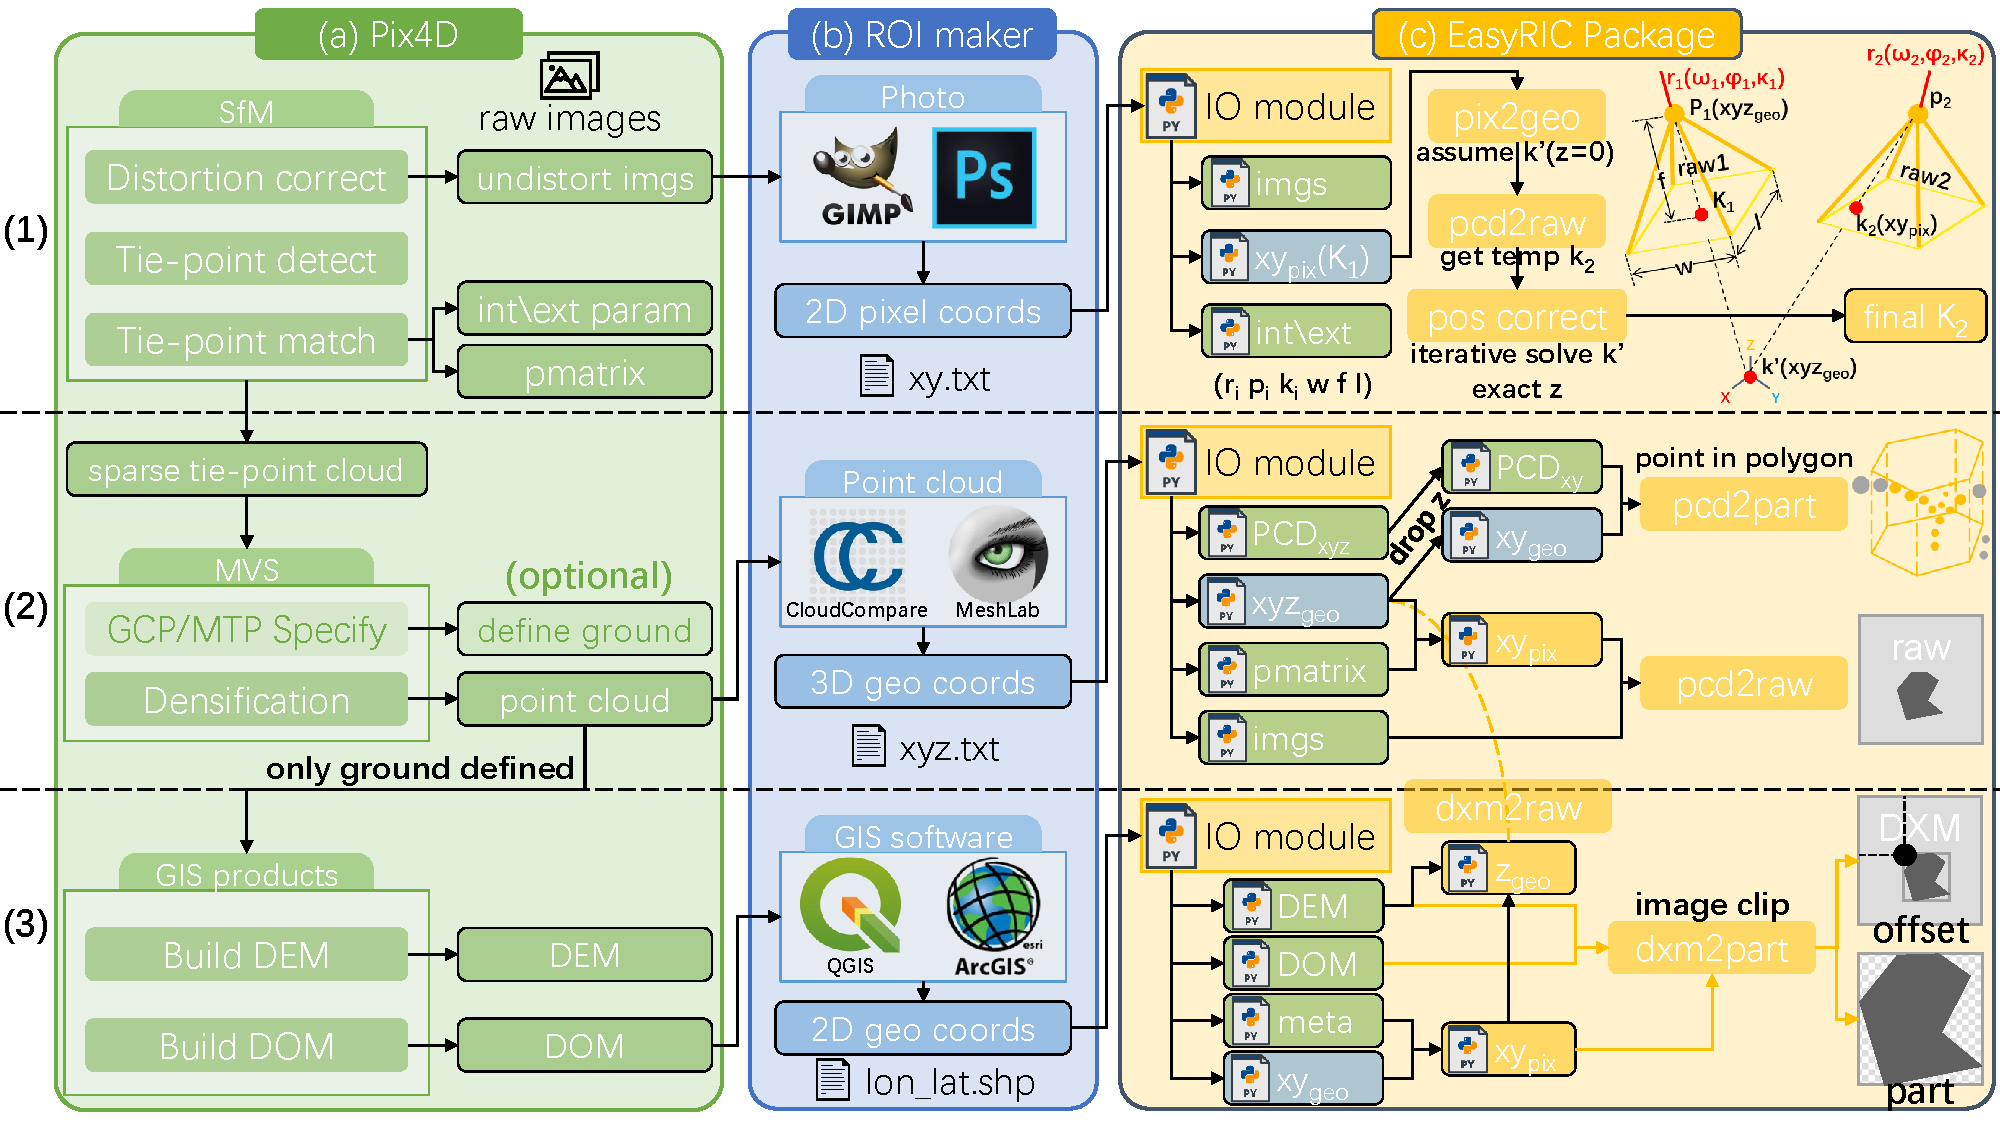
\includegraphics[width=0.95\linewidth]{figures/workflow.pdf}
  \caption{The workflow of proposed method. (\textbf{a}) The processing pipeline and output of 3D reconstruction (use Pix4Dmapper as example). This step can be separated into 3 parts: (1) the structure from motion (SfM) part which build the sparse tie-point cloud. (2) the multi-view stereo (MVS) photogrammetry part which densify previous sparse tie-point cloud and make geographic corrections. (3) For those defined ground plots, export \acrfull*{dom} and \acrfull*{dsm}. (\textbf{b}) The \acrfull*{roi} maker pipeline via commercial or open source tools. (\textbf{c}) The processing pipeline for EasyRIC package, (1) "2D to 2D" part (ROI from image 1 to image 2). $r_i$ represented camera rotation of image $i$; $p_i$, represented camera position of image $i$; $k_i$ represented 2D pixel coordinates on image $i$; $w$ was sensor width (mm); $f$ was sensor focal length, and $l$ was sensor length (mm). (2) "3D to 2D" part (ROI from point cloud data to raw images). (3) "2.5D to 2D part" (ROI from geographic shapefile to raw images)}
  \label{fig:workflow}
\end{figure}

\begin{figure}[!htb]
  %\centering
  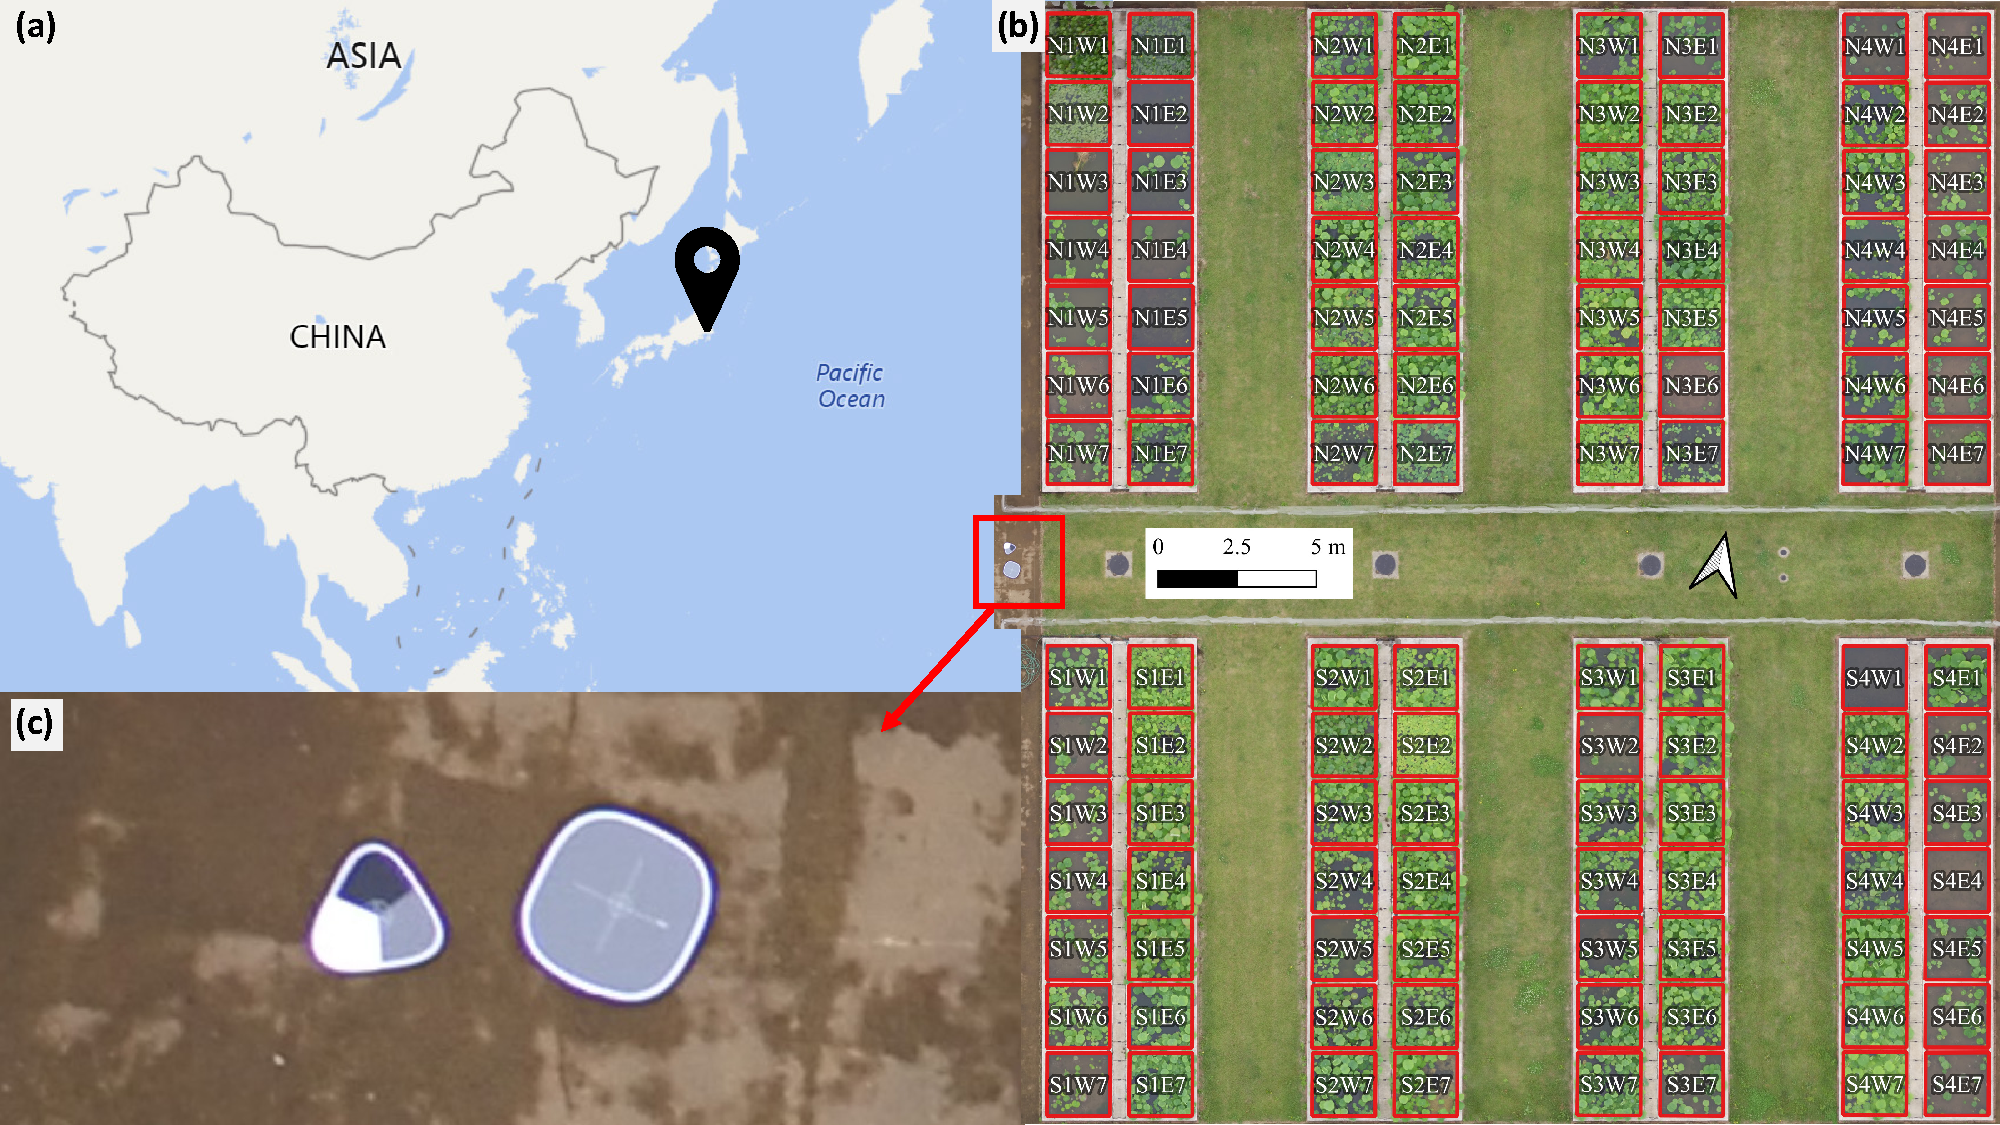
\includegraphics[width=0.95\linewidth]{figures/map.pdf}
  \caption{The experimental lotus plot condition. (\textbf{a}) the experimental plot locates in Nishi-Tokyo, Tokyo, Japan; (\textbf{b}) The labels of cultivation ponds, the orthomosaic showed here was collected on the May 5, 2017. The labels and boundaries of ponds were made by QGIS software and saved to shapefile (*.shp) for later usage; (\textbf{c}) shows the device used for obtaining geographic position and functioning as ground control point to linking different flight time series together}
  \label{fig:map}
\end{figure}

\begin{figure}[!htb]
  %\centering
  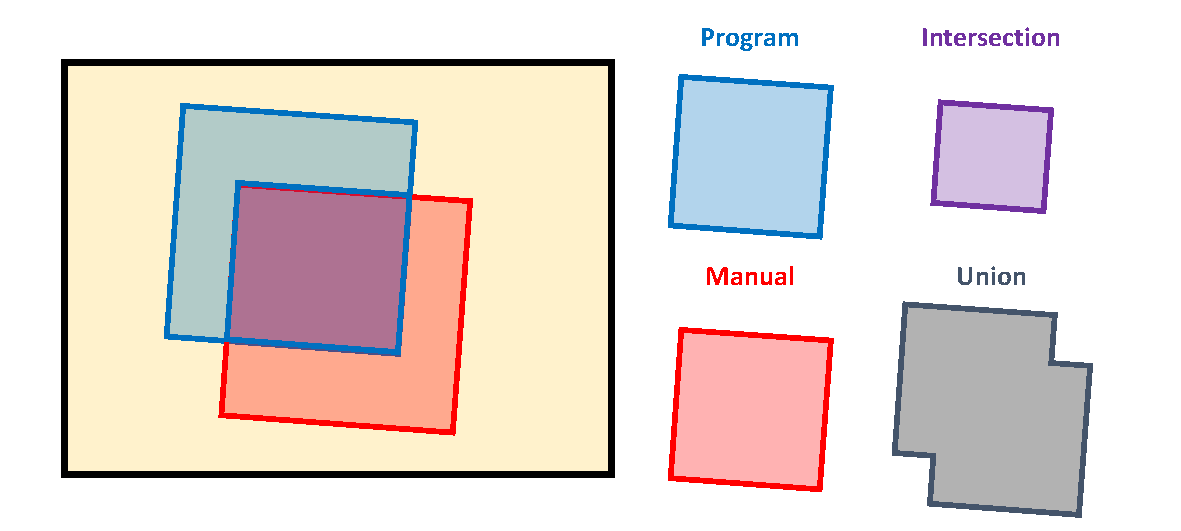
\includegraphics[width=0.95\linewidth]{figures/iou.pdf}
  \caption{The diagram of \acrfull*{iou} calculation. The red polygon is manual marking by LabelMe, the blue polygon is EasyRIC program calculated \acrfull*{roi} on raw images. The purple polygon is the intersection of two results while the gray polygon is the union of them. The IoU equals to the intersection divide by the union.}
  \label{fig:iou}
\end{figure}

\begin{figure}[!htb]
  %\centering
  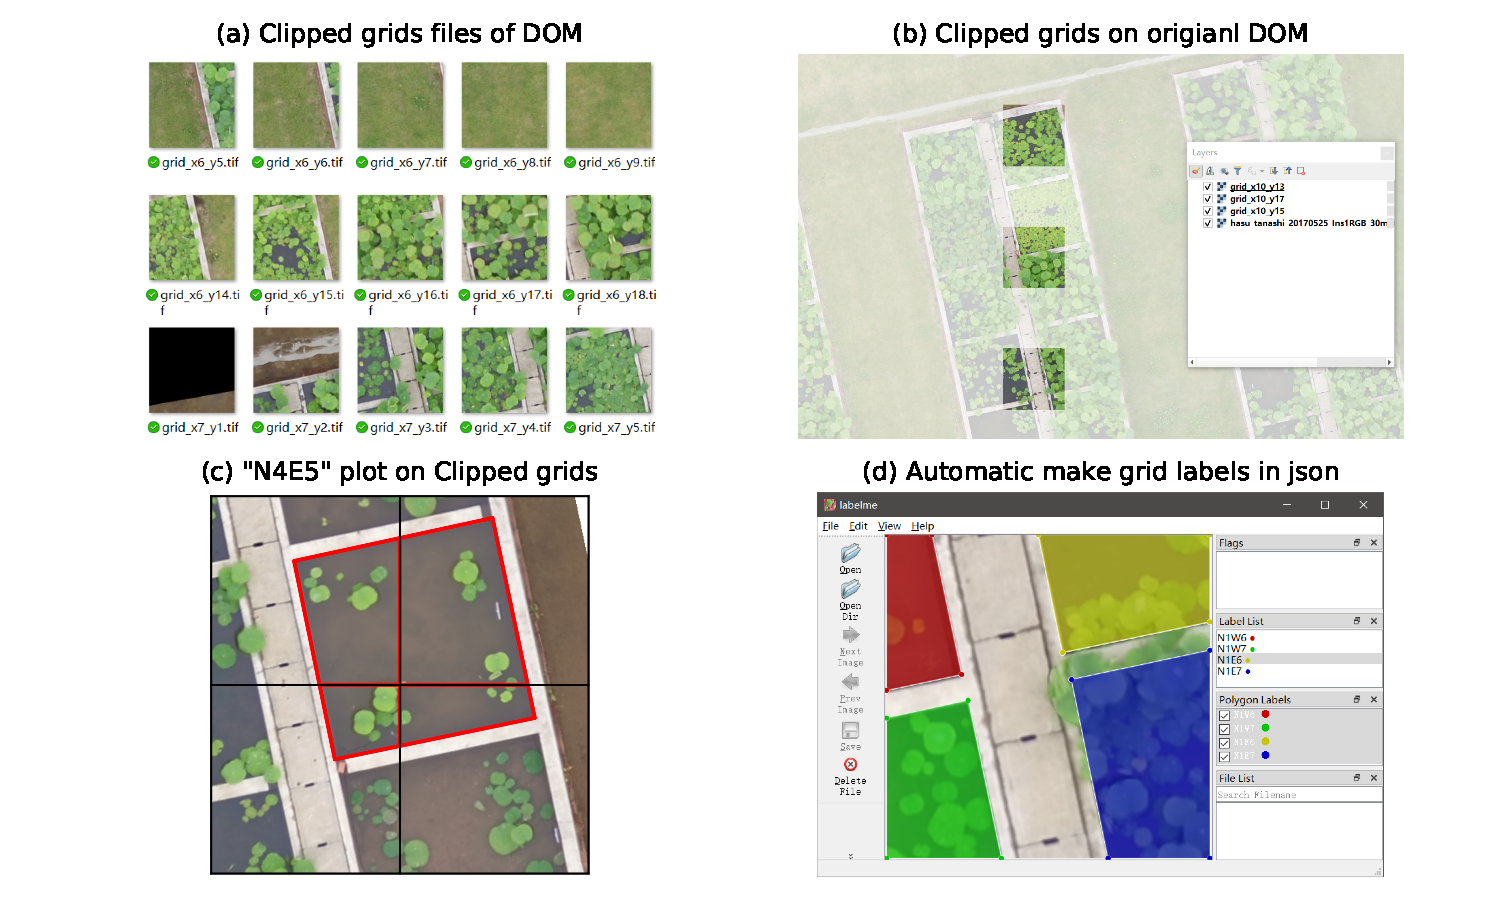
\includegraphics[width=0.95\linewidth]{figures/dom2grids.pdf}
  \caption{tbc}
  \label{fig:dom2girds}
\end{figure}

\begin{figure}[!htb]
  %\centering
  \includegraphics[width=0.95\linewidth]{figures/roi2dxm.pdf}
  \caption{tbc}
  \label{fig:roi2dxm}
\end{figure}

\begin{figure}[!htb]
  %\centering
  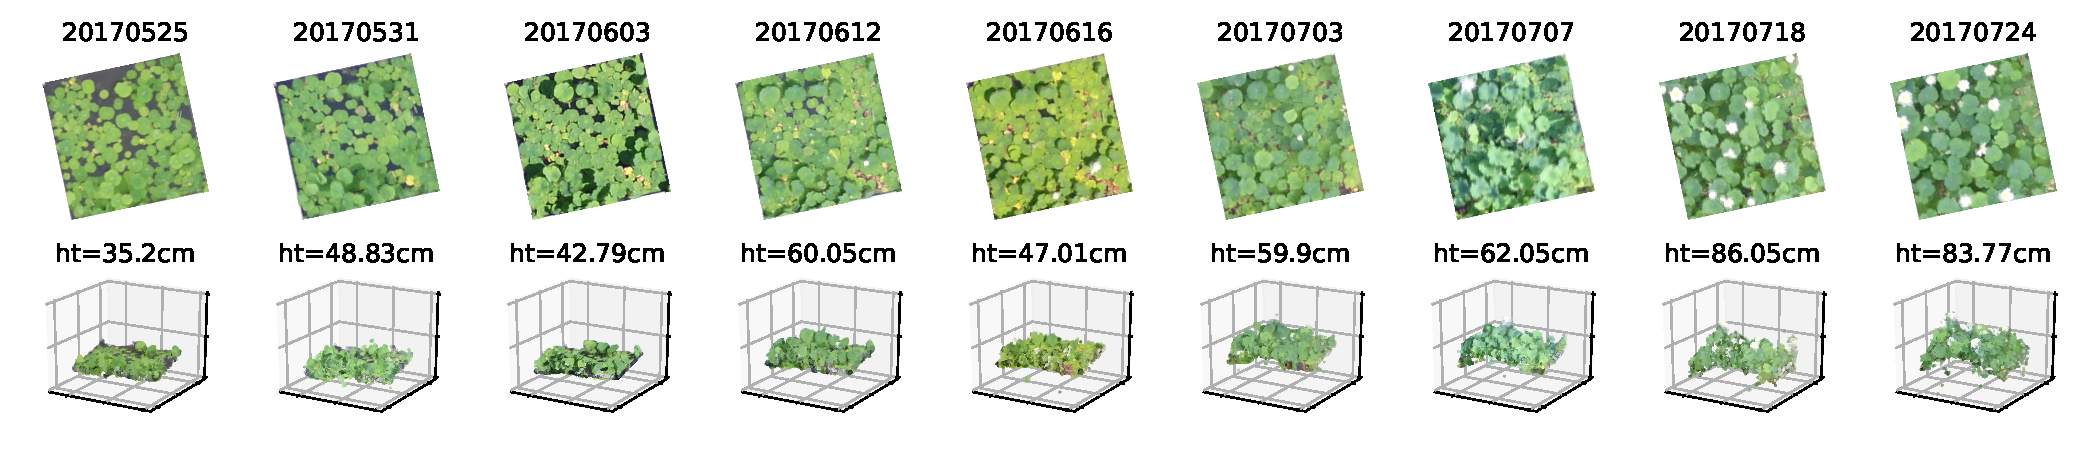
\includegraphics[width=0.95\linewidth]{figures/time_series.pdf}
  \caption{tbc}
  \label{fig:time}
\end{figure}


\begin{figure}[!htb]
  %\centering
  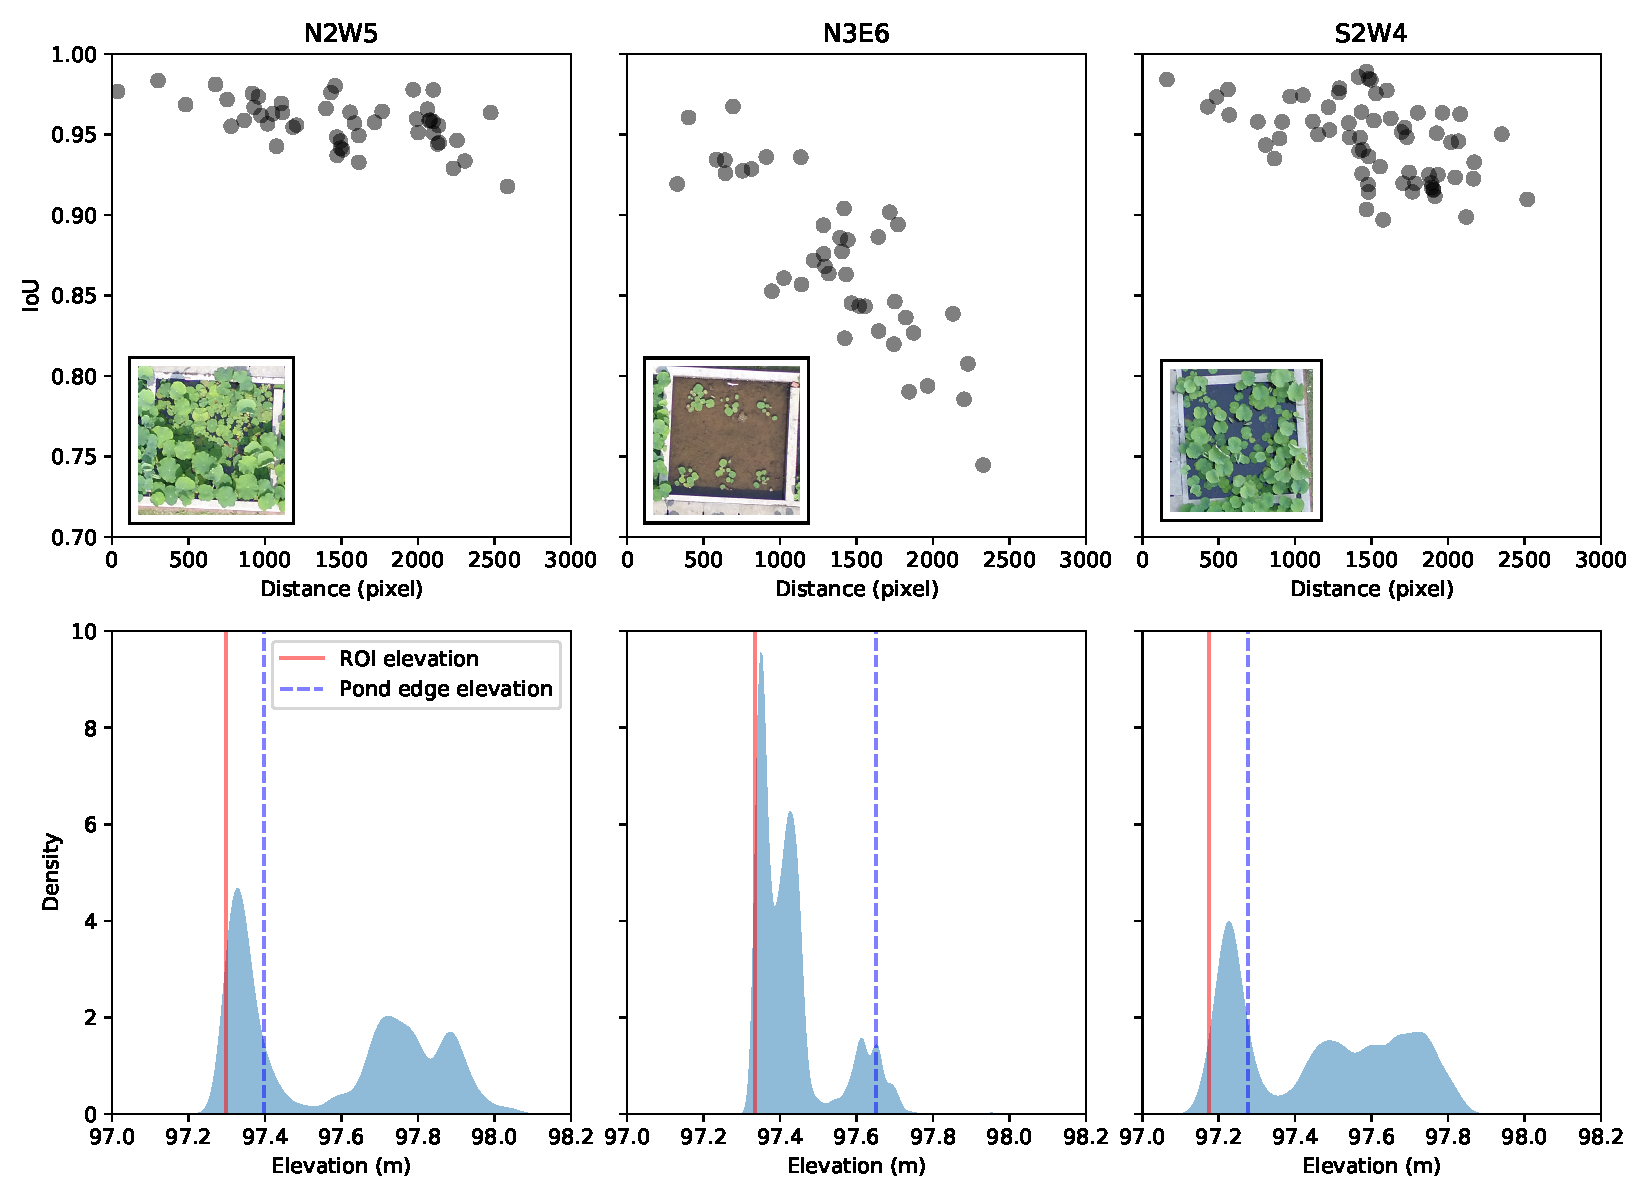
\includegraphics[width=0.95\linewidth]{figures/dist.pdf}
  \caption{tbc}
  \label{fig:dist}
\end{figure}

\begin{figure}[!htb]
  %\centering
  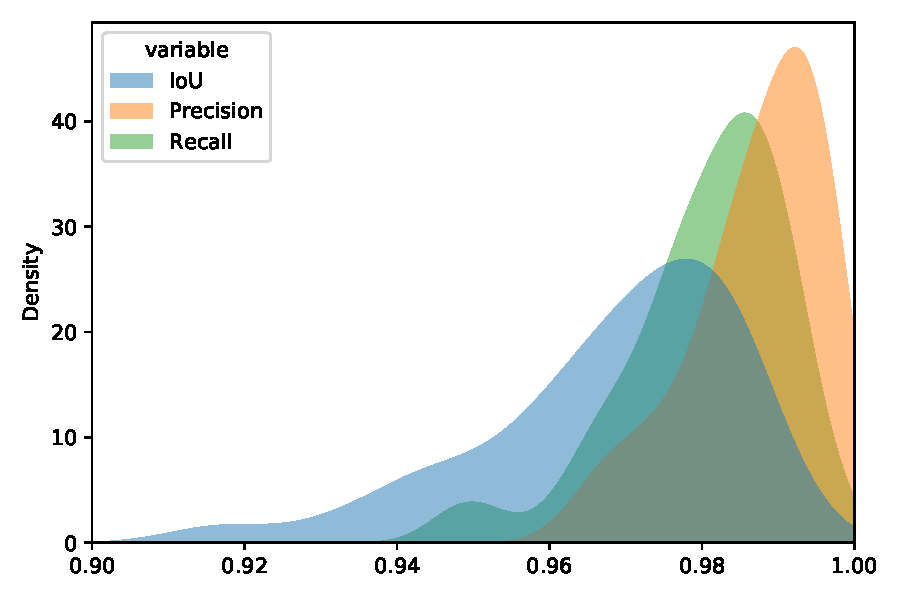
\includegraphics[width=0.95\linewidth]{figures/iou_all.pdf}
  \caption{tbc}
  \label{fig:iou_all}
\end{figure}

%%%%%%%%%%%%%%%%%%%%%%%%%%%%%%%%%%%
%%                               %%
%% Tables                        %%
%%                               %%
%%%%%%%%%%%%%%%%%%%%%%%%%%%%%%%%%%%

%% Use of \listoftables is discouraged.
%%
%\section*{Tables}

\begin{table}[!htb]
  \caption{Trail field and image collection information}
  \centering
  %% \tablesize{} %% You can specify the fontsize here, e.g., \tablesize{\footnotesize}. If commented out \small will be used.
  \resizebox{\textwidth}{!}{
  \begin{tabular}{ccccccc}
    \toprule
    \textbf{Flight date}	& \textbf{No. of raw images}	& \textbf{Size of raw images} & \textbf{Size of DOM} & \textbf{Size of DSM} & \textbf{Size of PCD}  & \textbf{Processing time} \\ 
    (yyyymmdd)&     & (GB) & (MB) & (MB) & (MB) & (min)\\
    \midrule
    20170525  & 266	& 1.64 & 38.5 & 34.6 & 89.2 & 39.7 \\
    20170531	& 151 & 0.94 & 40.4 & 37.6 & 60.0 & 47.3 \\
    20170603	& 141 & 0.87 & 46.5 & 34.1 & 60.3 & 18.8 \\
    20170612	& 285 & 1.74 & 38.1 & 32.9 & 93.8 & 101.5\\
    20170616	& 136 & 0.84 & 39.1 & 33.4 & 60.1 & 11.1 \\
    20170703	& 138 & 0.88 & 36.3 & 33.2 & 58.5 & 11.0 \\
    20170707	& 132 & 0.82 & 40.7 & 32.4 & 57.1 & 10.0 \\
    20170711	& 138 & 0.86 & 41.8 & 33.4 & 57.8 & 14.4 \\
    20170718	& 135 & 0.84 & 38.5 & 35.4 & 56.9 & 10.1 \\
    20170724	& 142 & 0.90 & 34.5 & 32.9 & 59.2 & 10.3 \\
    \bottomrule
  \end{tabular}
  }
  \label{tab:diginfo}
\end{table}

\end{backmatter}

\end{document}